\def\Yes{\text{Yes}}
\def\No{\text{No}}
\def\YesPrice{P(\Yes)}
\def\NoPrice{P(\No)}

\section{Theoretical Framework}

% TODO: Humanise
\subsection{Prediction Markets} \label{sec:prediction_markets}

Prediction markets are financial markets designed to forecast future events. Participants of prediction markets trade state-contingent claims whose payoff depends on how those future events unfold.
While different types of prediction markets have been designed, the scope of this thesis is limited to winner-take-all prediction markets. These markets are typically structured in the following way: a claim costs $\$p$ today and pays $\$1$ if and only if the stated event occurs, and $\$0$ otherwise. This structure implies two participants agreeing on the price $\$p$ which one of the participants pays, the other putting up $\$(1 - p)$, with the winner receiving "all" of the dollar put up in collateral as their payoff. \parencite{wolfers_prediction_2004}.
% Arrow-Debreu securities?
% The price $p$ can be read as the market-implied (risk-neutral) probability that the event happens, because the contract’s expected payoff equals p. Put differently, the price is a state price; under standard assumptions it coincides with the event’s probability. The same logic underlies families of related contracts (for example, across thresholds or outcomes), whose internal consistency and co-movement reflect how new information is incorporated through trading.

Through price discovery, traditional financial markets aggregate information about the value of assets. Prediction markets’ primary purpose is leveraging this role of markets for forecasting. Under the Efficient Markets Hypothesis, the market price on prediction markets should reflect the risk-neutral probabilities of the event in question, encompassing all available information.
\parencite{berg_prediction_2008}


% A winner-take-all example makes this concrete. Suppose there is a market on an election between two candidates, A and B. The contract “A wins” pays \$1 if A is elected, \$0 otherwise; likewise for “B wins.” In equilibrium, the “YES” price on A (say 0.62) is the market’s risk-neutral probability that A will win (62\%), and the “YES” price on B will be close to 1 - 0.62 = 0.38. If the two “YES” prices do not sum to one, arbitrageurs can buy the underpriced side(s) or sell the overpriced side(s) until prices realign, restoring probabilistic coherence and reinforcing information aggregation.
% Cite Wolfers and Zitzewitz
% Cite Seguillo


% In short, prediction markets function by turning beliefs about uncertain events into tradable payoffs; if EMH holds even approximately, the resulting prices are interpretable as expected values—risk-neutral probabilities in winner-take-all settings—making platforms like Polymarket natural objects for empirical study of price discovery.
% % Cite Wolfers and Zitzewitz
% % Cite Seguillo



% NOTE: Move to literature review or write literature review here?
% TODO: Elaborate
This efficiency and predictive power of prediction markets has been the topic
of vast existing literature, especially in the context of forecasting elections, such as in
\textcite{berg_prediction_2008} \textcite{erikson_are_2008}, who have found that .... 
% Empirical Berg (2008)
% Analytical Wolfers (2006)
This has also been tackled analytically, where \textcite{wolfers_interpreting_2006} derived two economic models which
describe sufficient conditions under which prediction markets prices correspond with participants' mean beliefs.
% Prediction markets were originally started by the Iowa State University for the 1988

% TODO: Write segue
However, little research has been done examining the world's largest prediction market as of 2025, Polymarket.
This is thesis aims to provide empirical research into the market efficiency of winner-take-all prediction markets 
in the context of markets focusing on the interest rate decisions of the US Federal Open Market Committee's (FOMC) following their scheduled meeting.

% TODO: Remove this when previous section written
\newpage

\subsection{Polymarket}


\subsubsection{Terminology}


% Figure out how to put this image where I want it to be
\begin{figure}[H]
  \begin{center}
    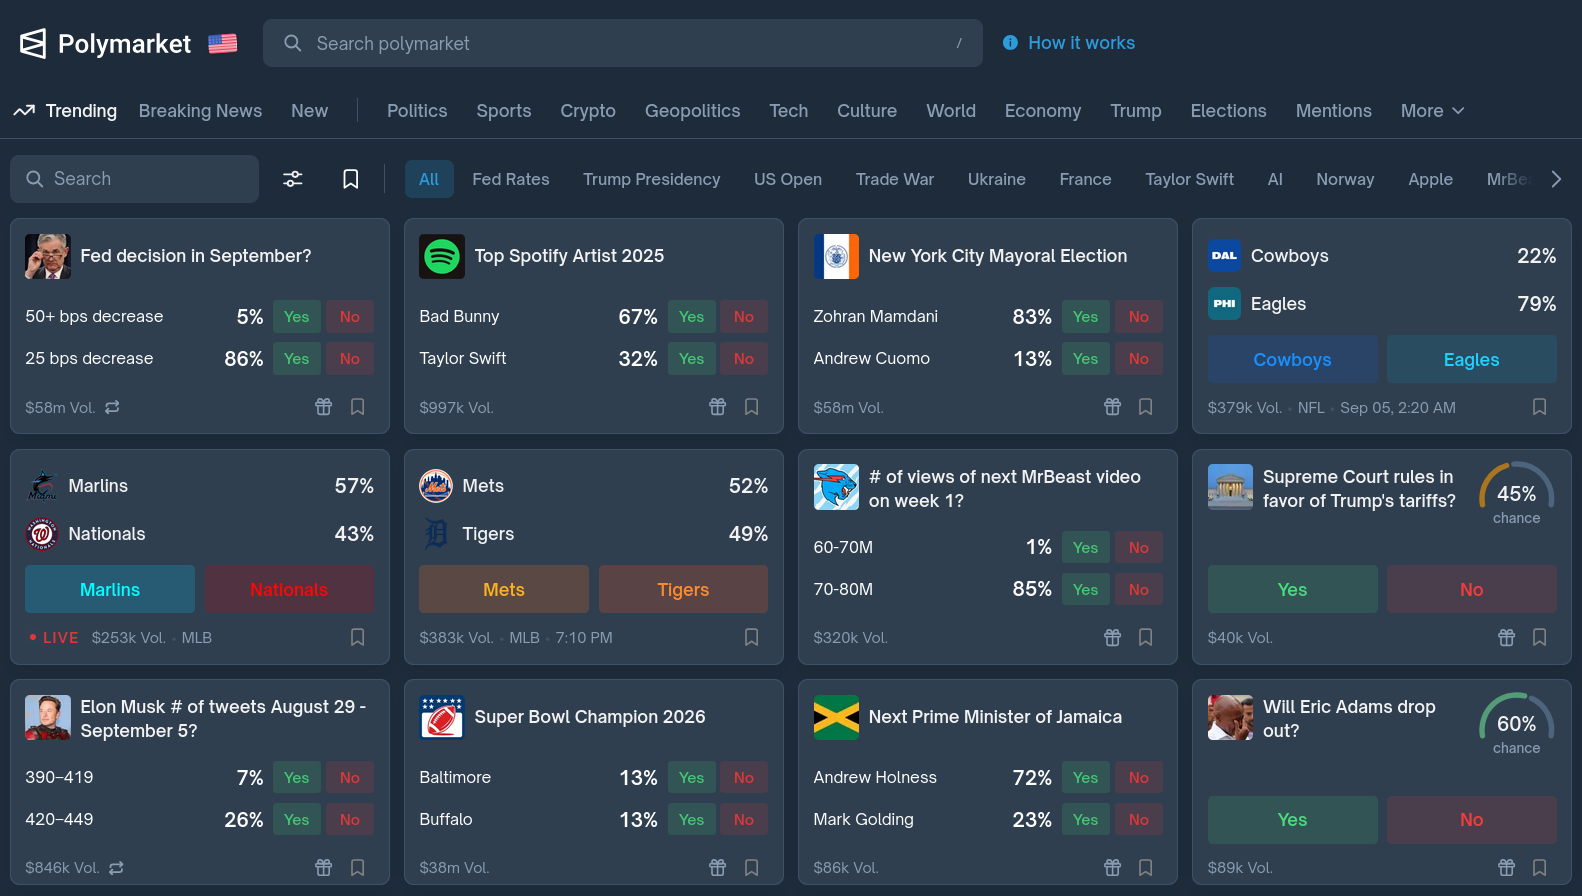
\includegraphics[width=0.95\textwidth]{figures/Polymarket_front_page.png}
  \end{center}
  \caption{The Polymarket front page as of September 3rd, 2025. While sports and politics events drive the highest volume, there are various events related to popular culture (\# of views of next MrBeast video, Top Spotify artist of 2025)}
  \label{fig:front_page}
\end{figure}


% Figure out how to put this image where I want it to be
\begin{figure}[H]
  \begin{center}
    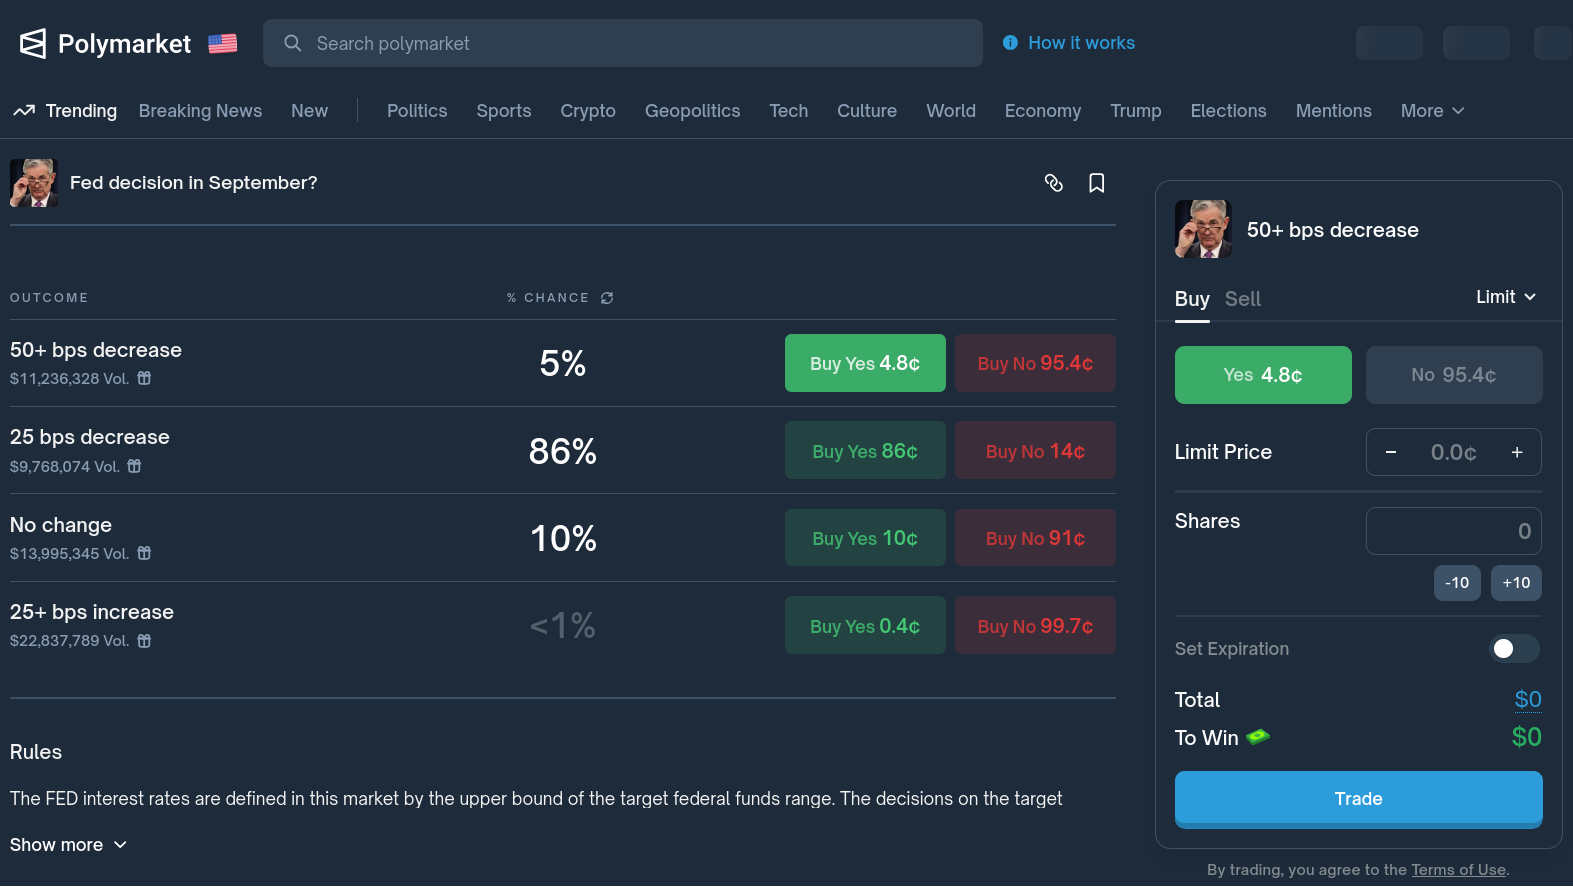
\includegraphics[width=0.95\textwidth]{figures/FOMC_event_September.png}
  \end{center}
  \caption{September FOMC event on Polymarket as of September 3rd, 2025}
  % FIX: this
  \caption*{Each market related to possible interest rate decisions (50+ bps increase, 25 bps decrease, No change, 25+ bps decrease) for the September FOMC meeting is grouped into its own event, making it easier for traders to compare prices. While buying both Yes and No shares is possible, shorting is not an option on Polymarket, which is why the cost of all the `Yes` claims exceeds \$1, and the cost of all `No` claims exceeds \$3.}
  \label{fig:FOMC_event_september}
\end{figure}


% FIX: Notation

Polymarket is the world's largest prediction market-hosting platform, % TODO: Source?
hosted on the website www.polymarket.com, and depicted in Figure \ref{fig:front_page}.
On Polymarket, prediction markets are grouped into `events`, which contain different `markets` related to a single topic/occasion.
While anyone can propose an event through social media channels such as Discord and Twitter/X, Polymarket retains the right to create events themselves.
Each `market` is a winner-take-all market as outlined in Section \ref{sec:prediction_markets}, and concerns itself with exactly one `question` regarding the outcome of the event it is a part of. Market participants can trade on these questions by buying or selling existing shares in binary `Yes` and `No` claims i.e. $C \in {\Yes, \No}$ (called `outcomes` or `outcome shares`), with prices for each of these shares, $P(C) \in \$[0, 1]$. % NOTE: delete duplicate
When an event concludes, its markets are 'resolved', meaning the claims of the outcome which realised in the world $C^*$ in each market can be converted to \$1 per claim, with claims in the opposite outcome, $C'$, realising a \$0 payoff.
This resolution happens according to `rules` stipulated for every event, which are designed to provide clarification on the markets' questions, in order to avoid situations where no market could resolve to a `Yes` outcome, despite being designed in such way.
\parencite{PMDocs}

Figure \ref{fig:FOMC_event_september} depicts the FOMC interest rate decision event for September, 2025, which features 4 markets regarding the potential interest rate decisions. These markets are non-overlapping and exhaustive, meaning one and only one of the markets will resolve to `Yes`, while the other markets resolve to `No`. This is ensured by the rules, which for this market are:

% September market rules
\begin{quote}
  {
    \smaller[1]
    \raggedright
    The FED interest rates are defined in this market by the upper bound of the target federal funds range. The decisions on the target federal fund range are made by the Federal Open Market Committee (FOMC) meetings.
    This market will resolve to the amount of basis points the upper bound of the target federal funds rate is changed by versus the level it was prior to the Federal Reserve's September 2025 meeting.
    If the target federal funds rate is changed to a level not expressed in the displayed options, the change will be rounded up to the nearest 25 and will resolve to the relevant bracket. (e.g. if there's a cut/increase of 12.5 bps it will be considered to be 25 bps)
    The resolution source for this market is the FOMC’s statement after its meeting scheduled for September 16 - 17, 2025 according to the official calendar:
    % \linebreak
    https://www.federalreserve.gov/monetarypolicy/fomccalendars.htm.

    The level and change of the target federal funds rate is also published at the official website of the Federal Reserve at
    % \linebreak
    https://www.federalreserve.gov/monetarypolicy/openmarket.htm.

    This market may resolve as soon as the FOMC’s statement for their September meeting with relevant data is issued. If no statement is released by the end date of the next scheduled meeting, this market will resolve to the "No change" bracket.
  }
\end{quote}


\subsubsection{Order Matching}

% Figure out how to put this image where I want it to be
\begin{figure}[H]
  \begin{center}
    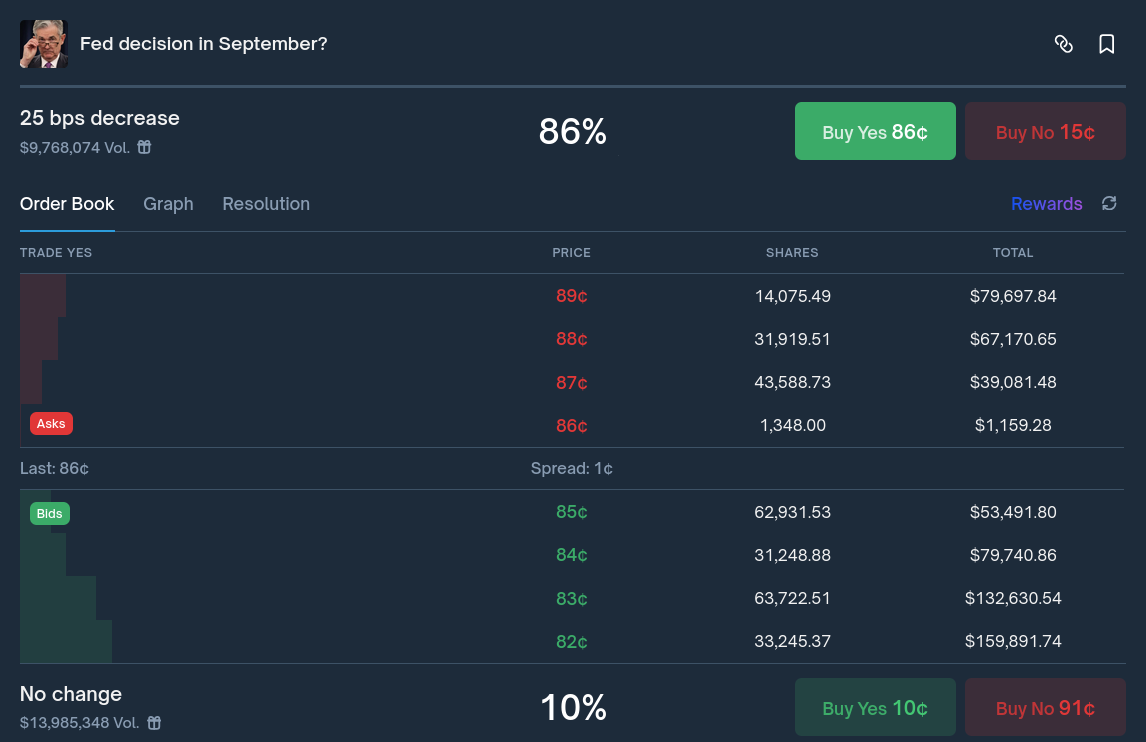
\includegraphics[width=0.95\textwidth]{figures/polymarket_continuous_double_auction_Yes.png}
  \end{center}
  \caption{The Polymarket front page as of September 3rd, 2025. While there is a variety of events, sports and politics markets are among the most popular}
  \label{fig:continuous_double_auction}
\end{figure}

% Figure out how to put this image where I want it to be
\begin{figure}[H]
  \begin{center}
    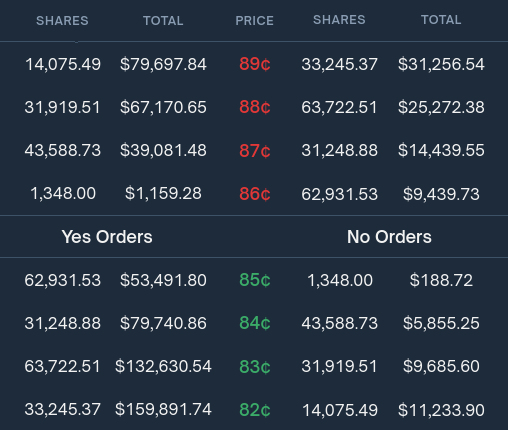
\includegraphics[width=0.95\textwidth]{figures/polymarket_orderbook.png}
  \end{center}
  % \caption{The Polymarket front page as of September 3rd, 2025. While there is a variety of events, sports and politics markets are among the most popular}
  % TODO: Add caption
% the 'total' displayed is cumulative, making this equivalence more difficult to spot for limit orders which are not the best bid or best ask.
  \label{fig:polymarket_orderbook}
\end{figure}

As Figure \ref{fig:FOMC_event_september} shows, market participants can submit limit or market orders to buy or sell Yes or No claims.
While buying is allowed at any quantity, short selling is not permitted on Polymarket, and only owned shares can be sold.
This results in some price-inefficiencies, such as in \ref{fig:FOMC_event_september}, where despite the exhaustive set of markets, for each market $i$ in the set of markets in that event, $I$, the bid prices exhibit $\sum_{i \in I} \YesPrice_{i} \ne \$1$, $\sum_{i \in I} \NoPrice_{i} \ne \$3$, as well as $\sum_{i \in I} (\YesPrice_{i} + \NoPrice_{i}) \ne \$4$. This, however, is not exploitable due to lack of short-selling.
As explained in Section \ref{sec:prediction_markets}, a trade is only possible if two individual market participants agree on a price, which is why on Polymarket, it is mechanically ensured that $\P(C) + P(C') = \$1$ for any two complementary claims (opposite outcomes).
This guarantees that every pair of claims $(C, C') \in {\Yes, \No}$ is necessarily fully collateralised by \$1, put up by the holders of the `Yes` and `No` shares, ensuring the successful resolution of the market. \parencite{PMDocs}

Trading on Polymarket takes form in a continuous double auction, with no halts in trading between a market's opening and its resolution.
This is shown in Figure \ref{fig:continuous_double_auction}, with resting bid and ask limit orders being displayed for `Yes` outcome claims in the market for the FOMC meeting in September to conclude with a 25 bps decrease in the upper bound of the target federal funds range.

Mechanically, this is realised on Polymarket's centralised limit order book (CLOB) which has a `hybrid` organisation of off-chain order matching, and on-chain settlement.
This entails that market participants' orders are submitted to the CLOB, hosted on Polymarket servers, where they are matched into trades. Once a trade has been recorded on the servers, the actual settlement, execution, and recording of transactions takes place on the Polygon blockchain.
While an in-depth description of the blockchain mechanism is beyond the scope of this thesis, the key implication is that all trades on Polymarket are publicly available, with identifiable users.
Internally, pairs of opposing outcome shares $(C, C')$ are represented by pairs of `binary outcome tokens`, which are pairs of $\Yes$ and $\No$ claims in the same market, created upon being exchanged for and collateralised by the same nominal amount of `USDC`, the underlying currency for all exchange taking place on Polymarket.
USDC is a cryptocurrency (a stablecoin), which is pegged to the United States dollar, and has been since 2021 accepted in transaction settlement by payment services provider Visa. \parencite{hussain_visa_2021}.
For the purposes of this thesis, `USDC` will be referred to in terms of US dollars (1 USDC = 1 USD), while the term `outcome token` may be used to refer to digital assets representing a single share in a claim.
The effects of Polymarket's internal mechanisms on data acquisition is elaborated on in Section \ref{sec:polymarket_data}.

There are three distinct possibilities by which market participants' orders are matched:

\paragraph{Direct trade} A marketable order (by a liquidity taker) in a given claim $C$ matches resting liquidity providing (maker) orders in the same claim $C$. Here, one side is selling the claim $C$, while their counterparty in the trade is buying that same claim.
Internally, settlement is a straightforward token-for-USDC swap at the matched price.
% On-chain, these transactions are recorded as `OrderFilled` events.
This order-matching mechanism is essentially identical to the one familiar from traditional equities markets.


\paragraph{Minting new tokens} Because a pair of opposite outcome tokens $(C, C')$ are always backed by \$1 of collateral,
two buy orders from opposite-token orderbooks can also be matched if they agree on the price.
In this case, new sets of binary outcome tokens are created, a process referred to as 'minting', where each pair of outcome tokens $(C, C')$ is backed by \$1 put up cumulatively by the counterparties of the trade.
Terminologically it can also be said that each dollar of collateral is 'split' into a pair of outcome tokens.
This happens when there exists a resting limit buy order (a bid) for the claim $C$ with price $P(C) =: p$, which is then matched with an incoming marketable buy (another bid) of the same size for the opposite claim $C'$ with price $P(C') = 1 - p$.

\paragraph{Burning tokens} The reverse operation of minting, this operation eliminates a set of outcome tokens $(C, C')$ from the market and releases the collateral which was used to back it.
This happens when two sell orders in opposite tokens' orderbooks sum such that the number of pairs of outcome tokens matches the amount of USDC cumulatively demanded, for them, i.e. when a resting sell order (an ask) for $C$ wishes to sell at price $P(C) =: p$, which is matched by an incoming marketable sell order of $C'$ of the same size at price $P(C') =: 1 - p$.
The set of tokens $(C, C')$ are burned (or 'merged'), and each side receives the collateral that had been initially put up when the tokens were minted.

Visually, as shown in Figure \ref{fig:polymarket_orderbook}, limit orders in orderbooks of a pair of outcome tokens $(C, C')$ are represented symmetrically, i.e. bids (resp. asks) in $C$ will be shown as asks (resp. bids) in $C'$, and vice versa. This follows the logic described above, since any of the three options for order matching appear the same to market participants.
Each of these order-matching mechanisms work based on the necessary condition that $P(C) + P(C') = \$1$, which underlies winner-take-all markets.
It is important to note that this is the only arbitrage-eliminating mechanism implemented internally, and that this only works on the level of markets, not events.
Since events are just collections of markets, there is no internal mechanism to prevent arbitrage across markets, such as
$\sum_{i \in I} \YesPrice_{i} \le \$1$, $\sum_{i \in I} \NoPrice_{i} \le \$N - 1$, as well as $\sum_{i \in I} (\YesPrice_{i} + \NoPrice_{i}) \le \$N$,
where $i$ is a market in the set of markets for a given event $I$ which contains $N$ number of markets.
\parencite{PMDocs, saguillo_unravelling_2025}

Additionally, the split/merge operations (minting and burning tokens) are not restricted to order matching.
Users may themselves at any time during the market's lifetime split units of USDC into pairs of binary outcome tokens $(C, C')$, 'buying' each for \$0.50, or merge a pair of tokens to receive the underlying collateral.
The former can be useful to market participants who wish to act as market makers, while the latter can be used to liquidate large positions over time without moving markets too heavily.

% However, split/merge operations need to be traded at some point to make a difference to the participant performing them. This means analysing transactions is sufficient.


% Put this where redemption is explained
% When the designated oracle finalizes the event’s outcome, the winning side is set to a payout of 1 while the losing side’s payout is 0. Holders of the winning token redeem by burning their positions for collateral via the contract’s redeem function. Because the system remained fully collateralized ex ante, there is no gap risk at resolution; the accounting identity closes as collateral is released to the winner and all losing tokens expire. This completes the contingent-claim lifecycle from issuance, through trading and inventory transformations, to settlement and redemption. ([Polymarket Documentation][8])


% TODO: Humanise
\subsection{Federal Funds Rate futures}

\subsubsection{Effective Federal Funds Rate (EFFR)}

The effective federal funds rate is the volume-weighted median interest rate on uncollateralised overnight loans of US dollar reserve balances between depository institutions in the United States. The Federal Reserve Bank of New York computes the EFFR and publishes it for the previous business day at approximately 9:00 a.m. New York time every day. This benchmark rate is the underlying asset of the Chicago Mercantile Exchange’s (CME's) 30-Day Federal Funds futures. \parencite{FED_EFFR_NY}


%%%%%%%%%%% UNREVIEWED TEXT STARTS HERE %%%%%%%%%%%
\subsubsection{Price quoting and the implied monthly average}

CME 30-Day Federal Funds (ZQ) futures are quoted in IMM index terms, with price equal to 100 minus the market-implied arithmetic average of daily EFFR over the contract’s calendar month. If the futures price for month T is $P_t^T$ (percent), the implied expected monthly average is

$$\mathbb{E}_t[\overline{r}_T] = 100 - P_t^T$$

where $\overline{r}_T$ denotes the arithmetic average of daily EFFR realizations during month $T$. This mapping follows directly from the contract’s price quotation and settlement definition.
% TODO: add citation for CME group's FedWatch methodology tool


\subsubsection{High-level assumptions for extracting probabilities}

To translate ZQ prices into probabilities of FOMC outcomes, the CME FedWatch methodology adopts three core assumptions.

First, rate changes occur in uniform 25-basis-point increments and the EFFR adjusts proportionally to the target change.

Second, within a meeting month, the EFFR is piecewise constant: it equals a pre-meeting level up to the decision’s effective date, and a post-meeting level thereafter.

Third, anchor months without FOMC meetings pin down a month-end/start-of-next-month level that is used to propagate boundary conditions through adjacent months. Under these assumptions, ZQ prices encode a risk-neutral expectation of the path of EFFR that can be decomposed into before/after segments in meeting months and rolled across months via anchors.
% TODO: add citation for CME group's FedWatch methodology tool

\subsubsection{Anchor months and boundary conditions}

In any month with no scheduled FOMC meeting, the entire calendar month is governed by a single policy regime, so the ZQ-implied average equals the expected EFFR throughout the month. FedWatch uses these months as anchors: for an anchor month $T$,

$$\text{EFFR(End)}_{T-1}=\text{EFFR(Avg)}_{T}=\text{EFFR(Start)}_{T+1}$$

Operationally, one identifies the nearest full non-meeting month, reads $\text{EFFR(Avg)}_{T}=100-P^T$ from its ZQ price, sets the end of the prior month and the start of the following month to that level, and then propagates these boundary values backward and forward as needed when solving adjacent meeting months. This anchoring step provides the initial conditions for the system of month-by-month equations.
% TODO: add citation for CME group's FedWatch methodology tool

\subsubsection{Meeting months and the time-weighting identity}

Consider a meeting month $T$ with $m_T$ calendar days and $k_T$ days before the policy change becomes effective. Let $r_T^{-}$ denote the pre-meeting EFFR level and $r_T^{+}$ the post-meeting level. Because the futures price reflects the arithmetic monthly average, the implied average satisfies the time-weighting identity

$$\mathbb{E}_t[\overline{r}_T] = \omega_T\, r_T^{-} + (1-\omega_T)\,\mathbb{E}_t[r_T^{+}], \qquad \omega_T \equiv \frac{k_T}{m_T}$$

Solving for the expected post-meeting level gives

$$\mathbb{E}_t[r_T^{+}] = \frac{m_T\,\mathbb{E}_t[\overline{r}_T] - k_T\, r_T^{-}}{m_T-k_T}$$

When the following month $T{+}1$ is an anchor, $\mathbb{E}_t[r_T^{+}]$ is identified directly from $\text{EFFR(Avg)}_{T+1}$. On the other hand, if the prior month is an anchor, $\,r_T^{-}$ is identified from $\text{EFFR(Avg)}_{T-1}$. In either case, the time-weighting identity links the observable ZQ-implied monthly average to the unobservable post-meeting level and enables sequential solution across the term structure.
% TODO: add citation for CME group's FedWatch methodology tool

\subsubsection{Probability calculations via the characteristic–mantissa method}

Define the expected change in EFFR over the meeting month as $\Delta_T^{*} \equiv \mathbb{E}_t[r_T^{+}] - r_T^{-}$. Express this in units of 25 bps, $\,n_T^{*} \equiv \Delta_T^{*}/0.25\%$. Decompose $n_T^{*}$ into its characteristic (integer) and mantissa (fractional) parts:

$$n_T^{*} = n_T + y_T,\qquad n_T \in \mathbb{Z}_{\ge 0}, 0 \le y_T < 1.$$

FedWatch interprets this as two mutually exclusive outcomes at the meeting: a change of $n_T \times 25$ bps with probability $1-y_T$, and a change of $(n_T{+}1)\times 25$ bps with probability $y_T$. When the expected change is less than one increment ($n_T=0$), this reduces to the familiar binomial case of no change versus a single 25-bp move with probabilities $1-y_T$ and $y_T$, respectively. In the special case where the next month is an anchor and one wishes to ask only “hike or hold by 25 bps,” the implied probability collapses to

$$\mathbb{P}(\text{25 bp hike})
= \frac{\text{EFFR(End)}_{T}-\text{EFFR(Start)}_{T}}{0.25\%},
\qquad
\mathbb{P}(\text{hold})=1-\mathbb{P}(\text{hike}),$$


%%%%%%%%%%% UNREVIEWED TEXT ENDS HERE %%%%%%%%%%%
